% A LaTeX (non-official) template for ISAE projects reports
% Copyright (C) 2014 Damien Roque
% Version: 0.2
% Author: Damien Roque <damien.roque_AT_isae.fr>

\documentclass[a4paper,12pt]{article}
\usepackage[utf8]{inputenc}
\usepackage[T1]{fontenc}
\usepackage[frenchb]{babel} % If you write in French
\usepackage{graphicx}
\usepackage{subfig}
\usepackage{tikz}
\usetikzlibrary{shapes,arrows}
\usepackage{pgfplots}
\pgfplotsset{compat=newest}
\pgfplotsset{plot coordinates/math parser=false}
\newlength\figureheight
\newlength\figurewidth
\pgfkeys{/pgf/number format/.cd,
set decimal separator={,\!},
1000 sep={\,},
}
\usepackage{ifthen}
\usepackage{ifpdf}
\ifpdf
\usepackage[pdftex]{hyperref}
\else
\usepackage{hyperref}
\fi
\usepackage{color}
\hypersetup{%
colorlinks=true,
linkcolor=black,
citecolor=black,
urlcolor=black}

\renewcommand{\baselinestretch}{1.05}
\usepackage{fancyhdr}
\pagestyle{fancy}
\fancyfoot{}
\fancyhead[LE,RO]{\bfseries\thepage}
\fancyhead[RE]{\bfseries\nouppercase{\leftmark}}
\fancyhead[LO]{\bfseries\nouppercase{\rightmark}}
\setlength{\headheight}{15pt}

\let\headruleORIG\headrule
\renewcommand{\headrule}{\color{black} \headruleORIG}
\renewcommand{\headrulewidth}{1.0pt}
\usepackage{colortbl}
\arrayrulecolor{black}

\fancypagestyle{plain}{
  \fancyhead{}
  \fancyfoot[C]{\thepage}
  \renewcommand{\headrulewidth}{0pt}
}

\makeatletter
\def\@textbottom{\vskip \z@ \@plus 1pt}
\let\@texttop\relax
\makeatother

\makeatletter
\def\cleardoublepage{\clearpage}
\makeatother

\usepackage{amsthm}
\usepackage{amssymb,amsmath,bbm}
\usepackage{array}
\usepackage{bm}
\usepackage{multirow}
\usepackage[footnote]{acronym}

\newcommand*{\SET}[1]  {\ensuremath{\mathbf{#1}}}
\newcommand*{\VEC}[1]  {\ensuremath{\boldsymbol{#1}}}
\newcommand*{\FAM}[1]  {\ensuremath{\boldsymbol{#1}}}
\newcommand*{\MAT}[1]  {\ensuremath{\boldsymbol{#1}}}
\newcommand*{\OP}[1]  {\ensuremath{\mathrm{#1}}}
\newcommand*{\NORM}[1]  {\ensuremath{\left\|#1\right\|}}
\newcommand*{\DPR}[2]  {\ensuremath{\left \langle #1,#2 \right \rangle}}
\newcommand*{\calbf}[1]  {\ensuremath{\boldsymbol{\mathcal{#1}}}}
\newcommand*{\shift}[1]  {\ensuremath{\boldsymbol{#1}}}

\newcommand{\eqdef}{\stackrel{\mathrm{def}}{=}}
\newcommand{\argmax}{\operatornamewithlimits{argmax}}
\newcommand{\argmin}{\operatornamewithlimits{argmin}}
\newcommand{\ud}{\, \mathrm{d}}
\newcommand{\vect}{\text{Vect}}
\newcommand{\sinc}{\ensuremath{\mathrm{sinc}}}
\newcommand{\esp}{\ensuremath{\mathbb{E}}}
\newcommand{\hilbert}{\ensuremath{\mathcal{H}}}
\newcommand{\fourier}{\ensuremath{\mathcal{F}}}
\newcommand{\sgn}{\text{sgn}}
\newcommand{\intTT}{\int_{-T}^{T}}
\newcommand{\intT}{\int_{-\frac{T}{2}}^{\frac{T}{2}}}
\newcommand{\intinf}{\int_{-\infty}^{+\infty}}
\newcommand{\Sh}{\ensuremath{\boldsymbol{S}}}
\newcommand{\C}{\SET{C}}
\newcommand{\R}{\SET{R}}
\newcommand{\Z}{\SET{Z}}
\newcommand{\N}{\SET{N}}
\newcommand{\K}{\SET{K}}
\newcommand{\reel}{\mathcal{R}}
\newcommand{\imag}{\mathcal{I}}
\newcommand{\cmnr}{c_{m,n}^\reel}
\newcommand{\cmni}{c_{m,n}^\imag}
\newcommand{\cnr}{c_{n}^\reel}
\newcommand{\cni}{c_{n}^\imag}
\newcommand{\tproto}{g}
\newcommand{\rproto}{\check{g}}
\newcommand{\LR}{\mathcal{L}_2(\SET{R})}
\newcommand{\LZ}{\ell_2(\SET{Z})}
\newcommand{\LZI}[1]{\ell_2(\SET{#1})}
\newcommand{\LZZ}{\ell_2(\SET{Z}^2)}
\newcommand{\diag}{\operatorname{diag}}
\newcommand{\noise}{z}
\newcommand{\Noise}{Z}
\newcommand{\filtnoise}{\zeta}
\newcommand{\tp}{g}
\newcommand{\rp}{\check{g}}
\newcommand{\TP}{G}
\newcommand{\RP}{\check{G}}
\newcommand{\dmin}{d_{\mathrm{min}}}
\newcommand{\Dmin}{D_{\mathrm{min}}}
\newcommand{\Image}{\ensuremath{\text{Im}}}
\newcommand{\Span}{\ensuremath{\text{Span}}}

\newtheoremstyle{break}
  {11pt}{11pt}%
  {\itshape}{}%
  {\bfseries}{}%
  {\newline}{}%
\theoremstyle{break}

\usetikzlibrary{arrows,shapes,snakes,automata,backgrounds,petri}
\newcommand{\hsp}{\hspace{20pt}}
\newcommand{\HRule}{\rule{\linewidth}{0.5mm}}



\title{ON : Rapport Projet}
\author{XAMBILI Robin}

\date{}


%Debut de ton document
\begin{document}
\makeatletter
  \begin{titlepage}
  \centering
      {\large \textsc{École Nationale Supérieure \\ d'Électrotechnique, d'Électronique, d'Informatique, \\ d'Hydraulique et des Télécommunications}}\\ \vspace{0.50cm}
      \textsc{Institut National Polytechnique}\\
    \vspace{1cm}
      
\includegraphics[width=0.7\textwidth]{img/n7.jpg}
  
    \vspace{3.5cm}
   % Title
    \HRule \\[0.3cm]
    { \huge \bfseries Traitement des données audiovisuelles : \\ \vspace{3mm} Rapport \\ 
    }
    \HRule \\[2cm]
    \vfill
    % Author
    \vspace{2em}
             
    \large XAMBILI Robin
    \vfill
	% Bas de page
	%\textsc{6 Novembre 2017}
    \newpage
    \renewcommand{\contentsname}{SOMMAIRE}
    \tableofcontents
  \end{titlepage}

%%%%%%%%%%%%%%%%%%%%%%%%%%%%%%%%%%%%%%%%%%%%
%%% Content of the report and references %%%
%%%%%%%%%%%%%%%%%%%%%%%%%%%%%%%%%%%%%%%%%%%%

\section{Introduction}
\newpage


\section{TP01 : Espaces de représentations des couleurs}

\subsection{Corrélations et contraste des canaux RVB}

Le script \textbf{exercice1.m} lit une image codée en RVB (autumn.tif) et affiche l'image ainsi que les trois canaux RVB. On peut ainsi remarquer que les trois canaux sont fortement corrélés (l'affichage des trois canaux se ressemblent). Le calcul des coefficients de corrélation linéaire vient confirmer cette observation visuelle. De plus, les canaux sont tous visuellement assez peu contrastés. Cela est bien reflété par le calcul de la proportion de contraste de chaque canal.

\begin{figure}[htbp]
	\centering
	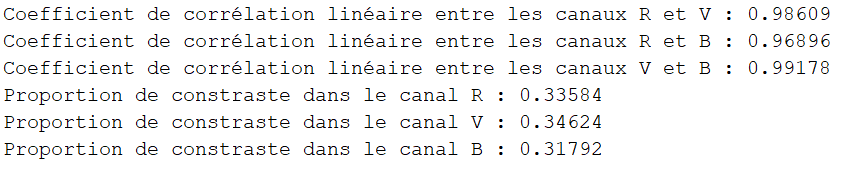
\includegraphics{img/TP1_ex1_res.PNG}
	\caption{Coefficients de corrélation linéaire et proportion de contraste des canaux RVB de l'image autumn.tif}
\end{figure}

\begin{figure}[htbp]
	\centering
	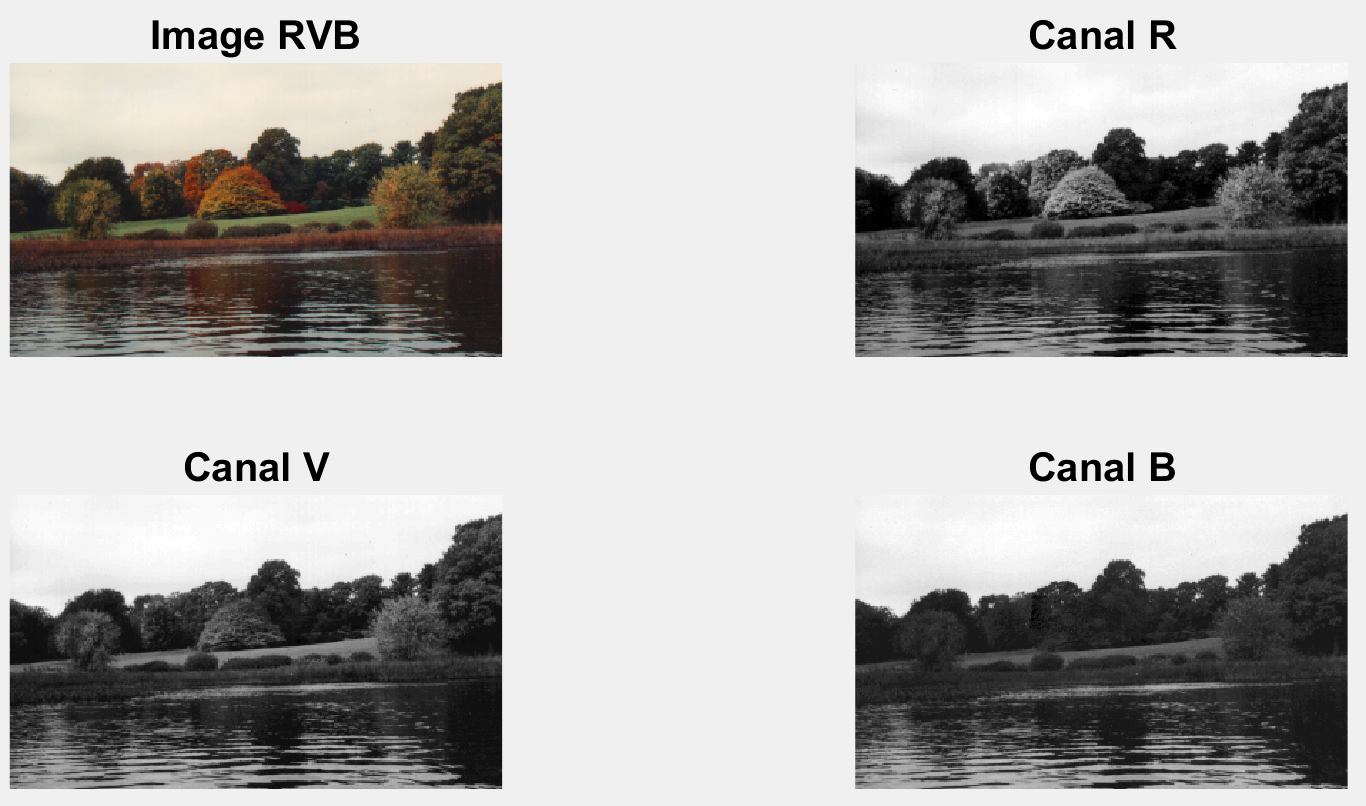
\includegraphics[scale=0.47]{img/TP1_ex1_figure_autumn.PNG}
	\caption{Canaux R,V et B de l'image autumn.tif}
\end{figure}

\newpage
\subsection{Transmission d'une image couleur par un seul canal}

Pour transmettre une image couleur par un seul canal, suffirait-il de transmettre le canal R,V ou B choisi arbitrairement? Si l'on compare les différents canaux à l'image couleur gantrycrane.png (cf. figure 3) le visuel n'est pas le même suivant le canal choisi. En effet, pour les canaux et R et V le visuel donne l'impression que le ciel est foncé et il semble faire nuit. Ici, le visuel le plus satisfaisant est le canal B ce qui correspond à la proportion de contraste la plus élevée : 74\%. Il semble donc plus pertinent de choisir le canal avec la plus grande proportion de contraste.
Cependant, comment faire lorsque les proportions de contraste des canaux sont très rapprochées comme pour autumn.tif ?


\begin{figure}[htbp]
	\centering
	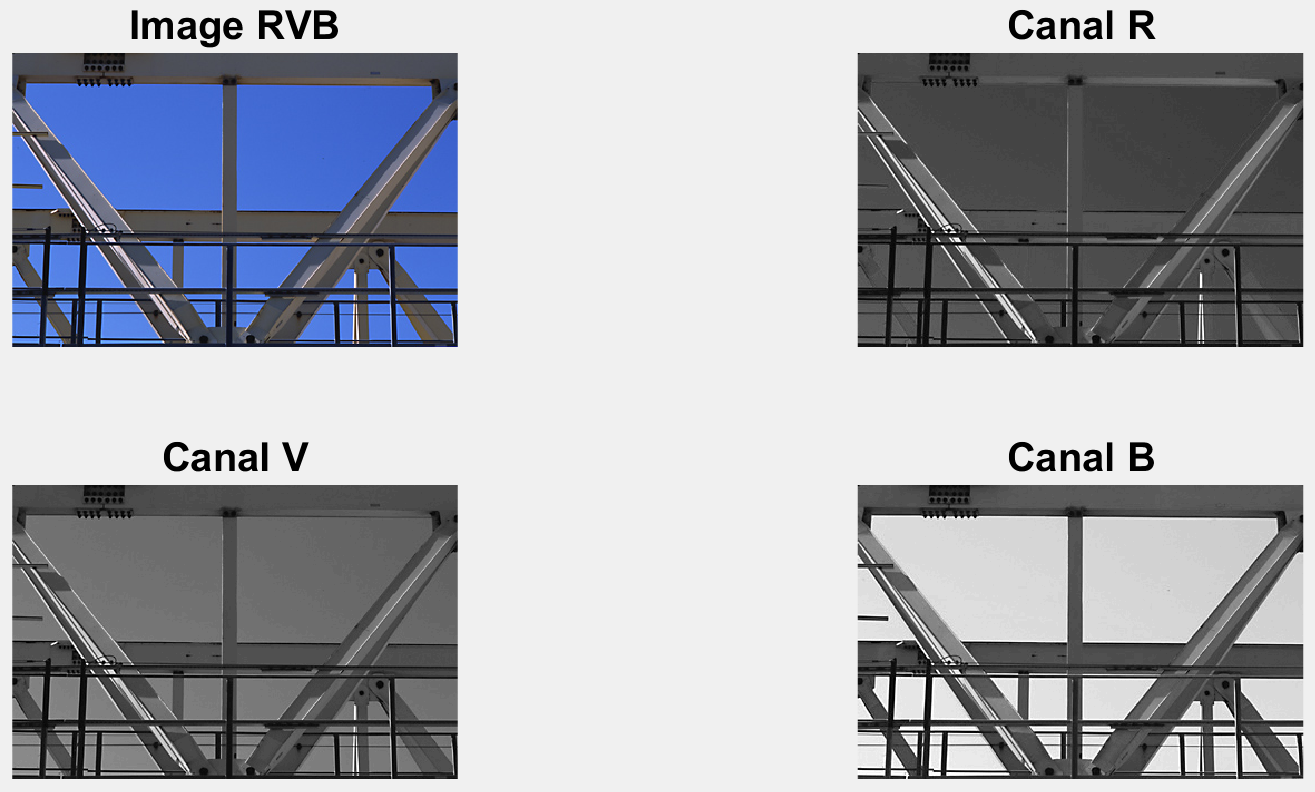
\includegraphics[scale=0.55]{img/TP1_ex1_figure_gantrycrane.PNG}
	\caption{Canaux R,V et B de l'image gantrycrane.png}
\end{figure}

\begin{figure}[htbp]
	\centering
	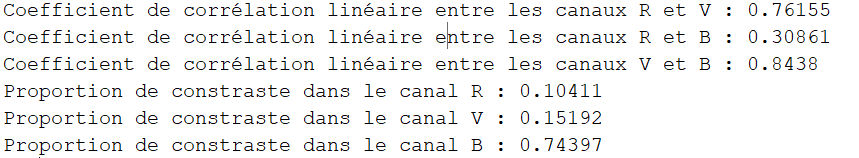
\includegraphics{img/TP1_ex1_res2.PNG}
	\caption{Coefficients de corrélation linéaire et proportion de contraste des canaux RVB de l'image gantrycrane.png}
\end{figure}

\subsection{Analyse en composantes principales}

Si le critère retenu est celui du contraste, l'ACP est le meilleur moyen de convertir une image couleur en une image en niveaux de gris. En effet, la première composante principale a le visuel le plus fidèle à l'image originale et la proportion de contraste de la première composante principale est plus élevée que celle des autres composantes ainsi que des canaux RVB.

\begin{figure}[htbp]
	\centering
	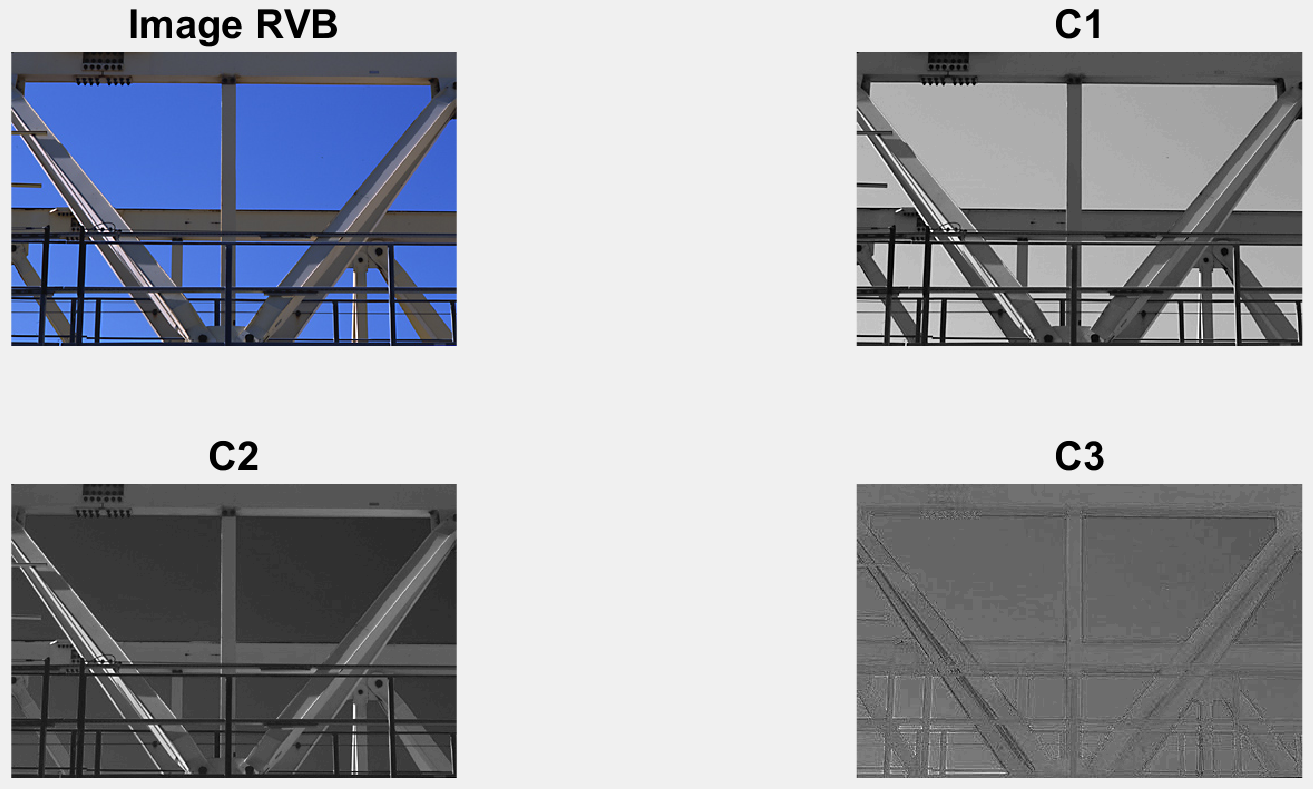
\includegraphics[scale=0.6]{img/TP1_ex2_figure_gantrycrane.PNG}
	\caption{Séparation des composantes principales de l'image gantrycrane.png}
\end{figure}

\begin{figure}[htbp]
	\centering
	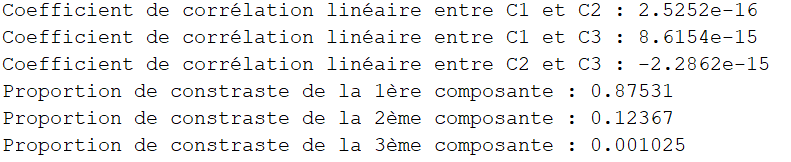
\includegraphics{img/TP1_ex2_res.PNG}
	\caption{Coefficients de corrélation linéaire et proportion de contraste des composantes principales de l'image gantrycrane.png}
\end{figure}
\newpage

\subsection{Combinaisons linéaire des trois canaux RVB}

La matrice de passage de l'ACP dépendant de l'image considérée, une matrice de passage commune à toutes les images a été choisie dans les années 1960.

Les différentes transformations sont plus ou moins satisfaisantes suivants le type d'images : 
\begin{itemize}
\item[•] Sur les images avec un canal B de proportion de contraste prédominant comme gantrycrane.png, la composante principale de l'ACP semble avoir le meilleur contraste.
\item[•] Sur les images très colorées comme coloredChips.png, la combinaison linéaire (2) semble mieux contraster certaines couleurs, notamment le jaune et le bleu, cependant certaines couleurs comme le rouge et le vert sont plus difficilement différentiables.
\item[•] Sur les images avec les canaux RVB de proportions de contrastes assez proches, les trois transformations sont très semblables.
\end{itemize}

\begin{figure}[htbp]
	\centering
	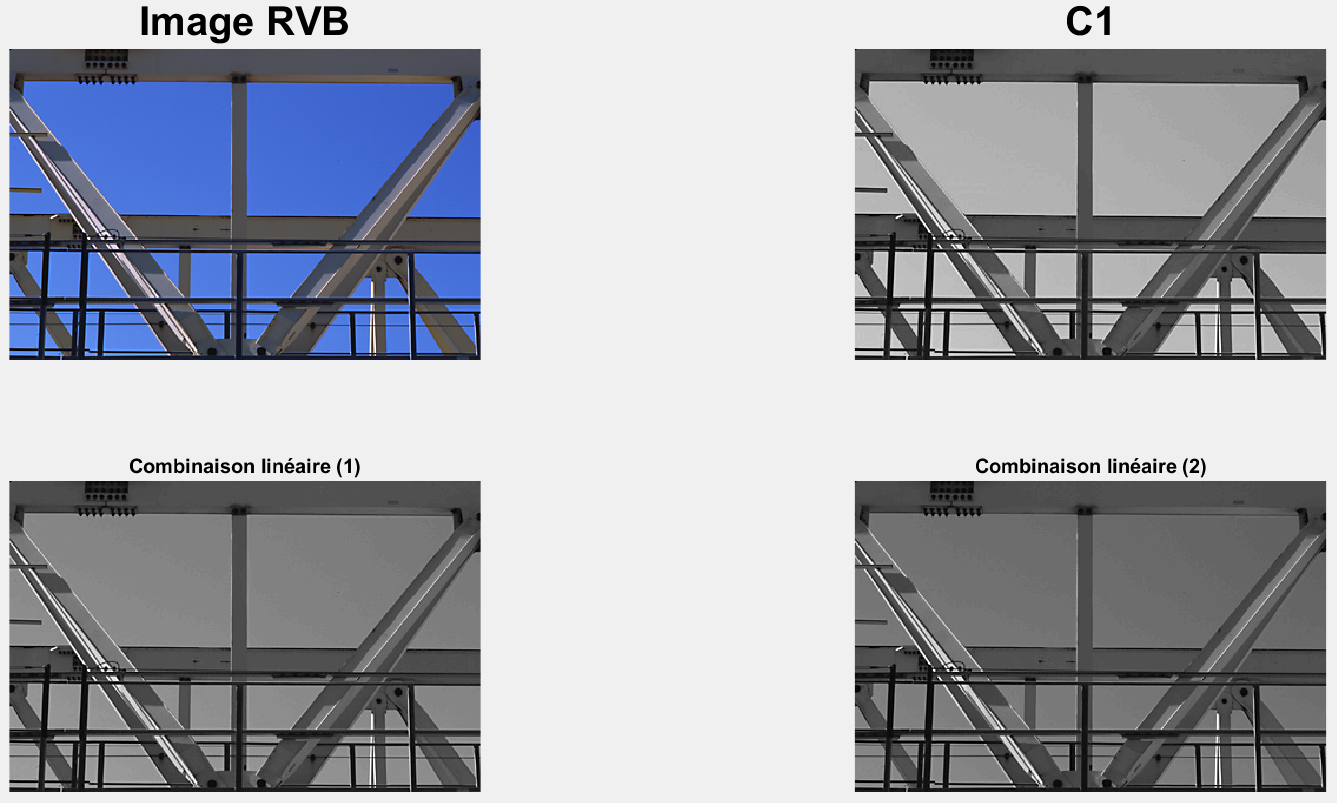
\includegraphics[scale=0.55]{img/TP1_ex3_figure_gantrycrane.PNG}
	
	\caption{Différentes combinaisons linéaires des canaux RVB}
\end{figure}

\begin{figure}[htbp]
	\centering
	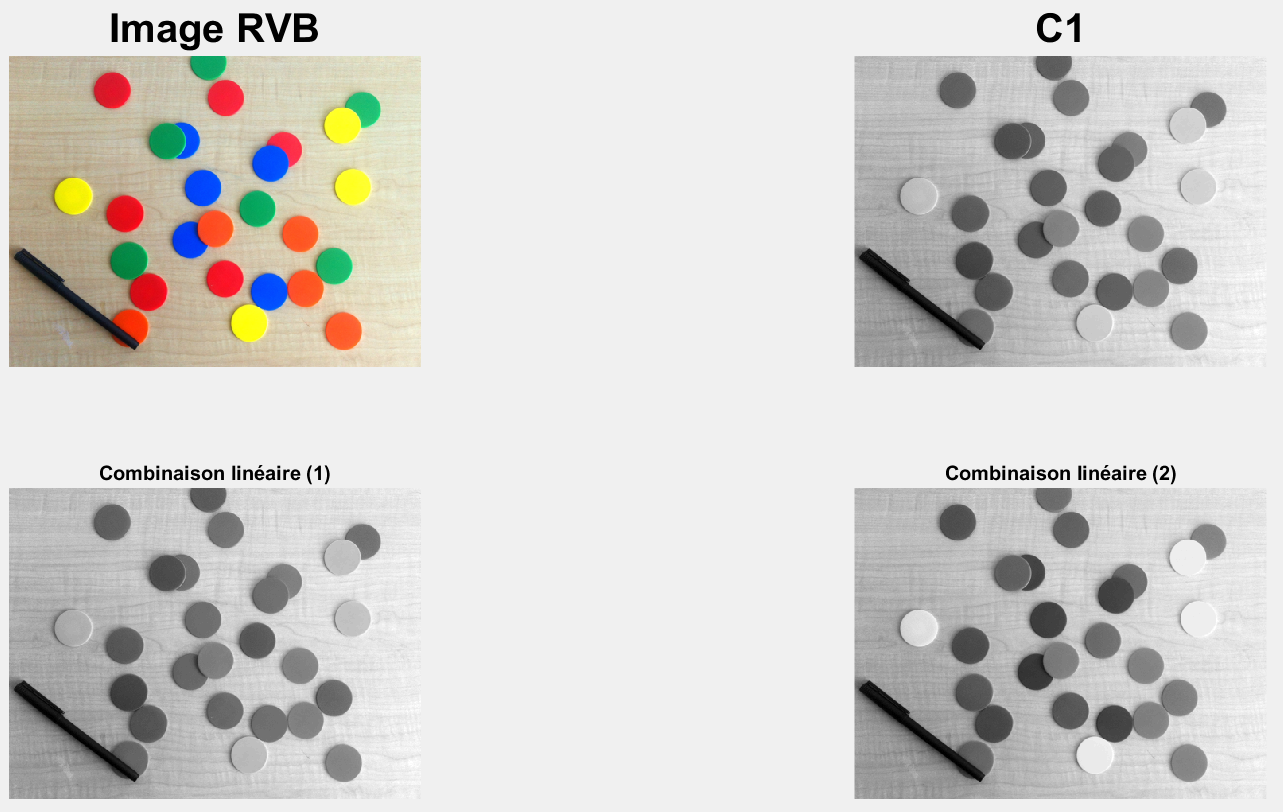
\includegraphics[scale=0.55]{img/TP1_ex3_figure_coloredChips.PNG}
	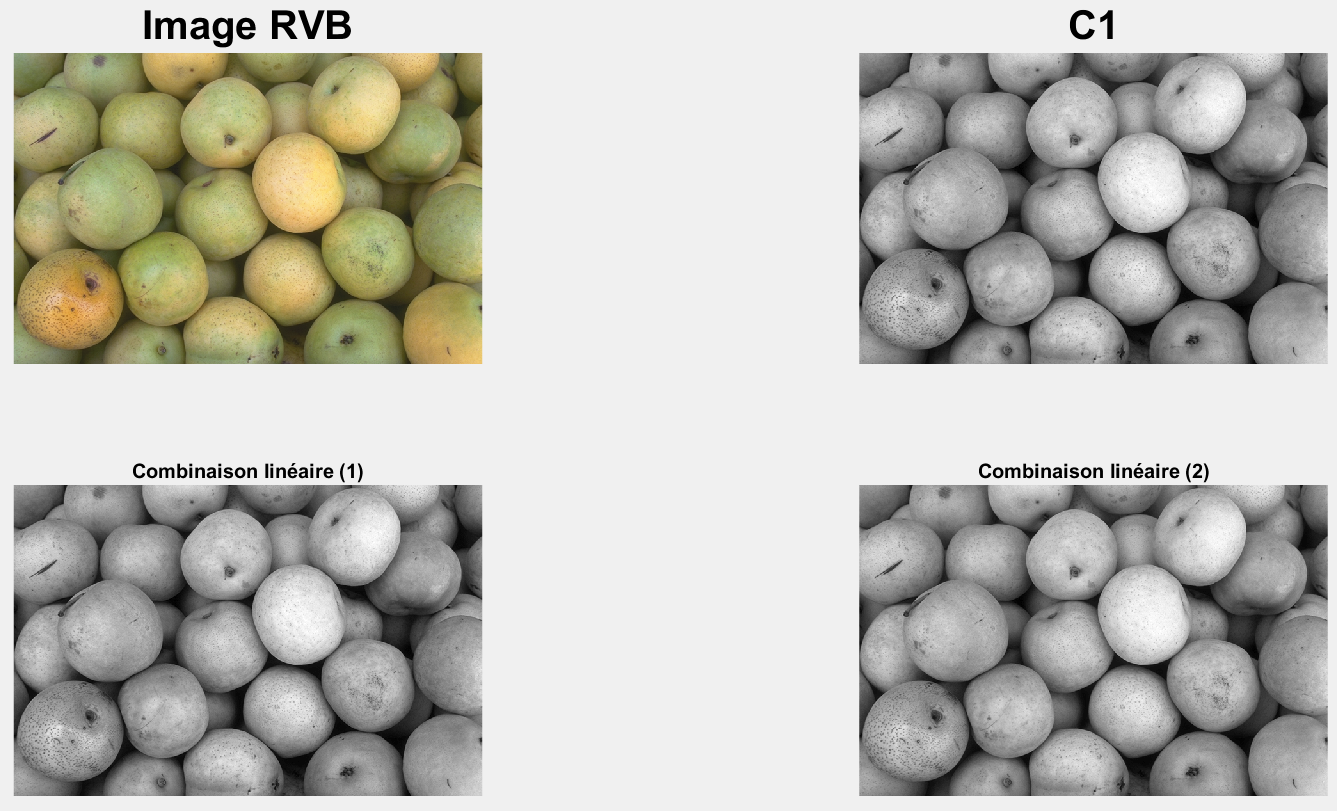
\includegraphics[scale=0.55]{img/TP1_ex3_figure_pears.PNG}
	\caption{Différentes combinaisons linéaires des canaux RVB}
\end{figure}

\end{document}